% !TeX spellcheck = cs_CZ
%{\tikzset{external/prefix={tikz/FYZII/}}
% \tikzset{external/figure name/.add={ch39_}{}}
%---------------------------------------------------------------------------------------------------
% file fey2ch39.tex
%---------------------------------------------------------------------------------------------------
%=========================== Kapitola Pružné látky =================================================
\setchaptertoc
\chapter{Pružné látky}\label{fyz:IIchapIXL}

  \section{Tenzor deformace}\label{fyz:IIchapIXLsecI}
  \section{Tenzor pružnosti}\label{fyz:IIchapIXLsecII}
  \section{Pohyby v pružném tělese}\label{fyz:IIchapIXLsecIII}
  \section{Nepružné chování}\label{fyz:IIchapIXLsecIV}
  \section{Výpočet konstant pružnosti}\label{fyz:IIchapIXLsecV}

    \begin{figure}[ht!]
      \centering
      \subcaptionbox{\label{fyz:fig0788a}}{\luafigure[0.9]{fyz_fig0788a.pdf}}               \\
      \subcaptionbox{\label{fyz:fig0788b}}{\luafigure[0.9]{fyz_fig0788b.pdf}}
      \label{fyz:fig0788}
      \caption{
               (\cite[s.~748]{Feynman02})}
    \end{figure}

    \begin{figure}[ht!] %\ref{fyz:fig0789}
      \centering
      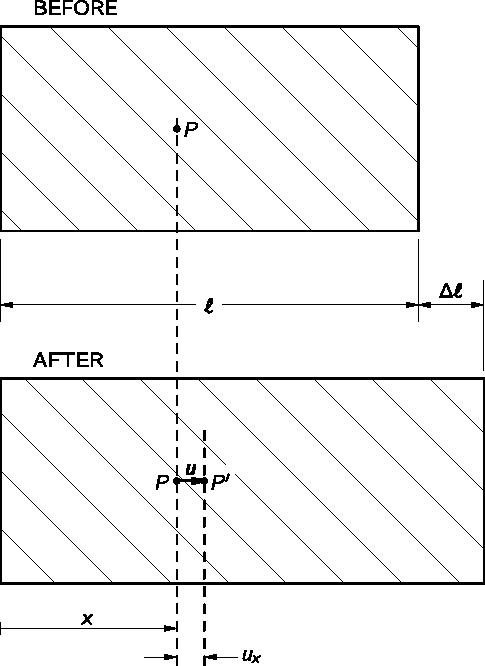
\includegraphics[width=0.7\linewidth]{fyz_fig0789.pdf}
      \caption{
               (\cite[s.~707]{Feynman02})}
      \label{fyz:fig0789}
    \end{figure}

    \begin{figure}[ht!]
      \centering
      \subcaptionbox{\label{fyz:fig0790a}}{\luafigure[0.9]{fyz_fig0790a.pdf}}               \\
      \subcaptionbox{\label{fyz:fig0790b}}{\luafigure[0.9]{fyz_fig0790b.pdf}}
      \label{fyz:fig0790}
      \caption{
               (\cite[s.~748]{Feynman02})}
    \end{figure}

    \begin{figure}[ht!]
      \centering
      \subcaptionbox{\label{fyz:fig0791a}}{\luafigure[0.9]{fyz_fig0791a.pdf}}               \\
      \subcaptionbox{\label{fyz:fig0791b}}{\luafigure[0.9]{fyz_fig0791b.pdf}}
      \label{fyz:fig0791}
      \caption{
               (\cite[s.~748]{Feynman02})}
    \end{figure}

    \begin{figure}[ht!] %\ref{fyz:fig0792}
      \centering
      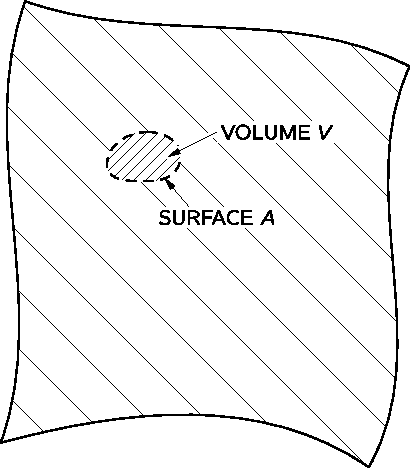
\includegraphics[width=0.7\linewidth]{fyz_fig0792.pdf}
      \caption{
               (\cite[s.~707]{Feynman02})}
      \label{fyz:fig0792}
    \end{figure}

    \begin{figure}[ht!] %\ref{fyz:fig0793}
      \centering
      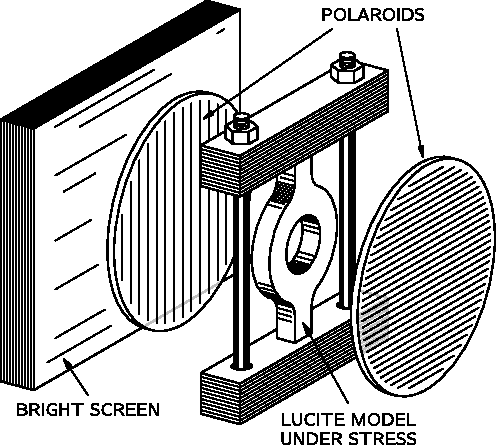
\includegraphics[width=0.7\linewidth]{fyz_fig0793.pdf}
      \caption{
               (\cite[s.~707]{Feynman02})}
      \label{fyz:fig0793}
    \end{figure}

    \begin{figure}[ht!] %\ref{fyz:fig0794}
      \centering
      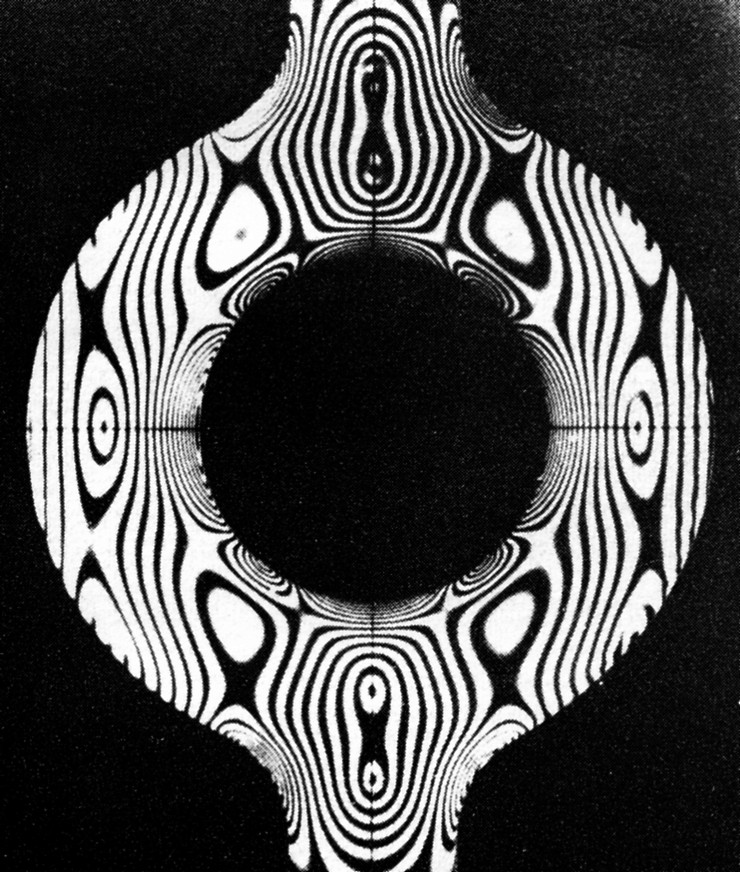
\includegraphics[width=0.7\linewidth]{fyz_fig0794.jpg}
      \caption{
               (\cite[s.~707]{Feynman02})}
      \label{fyz:fig0794}
    \end{figure}

    \begin{figure}[ht!] %\ref{fyz:fig0795}
      \centering
      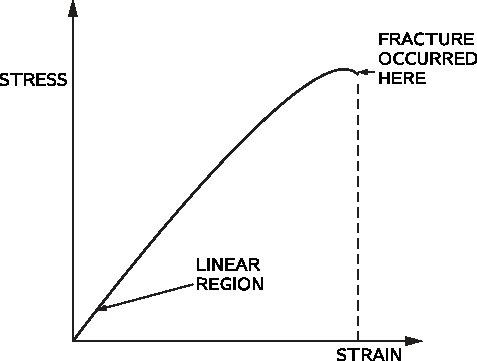
\includegraphics[width=0.7\linewidth]{fyz_fig0795.pdf}
      \caption{
               (\cite[s.~707]{Feynman02})}
      \label{fyz:fig0795}
    \end{figure}

    \begin{figure}[ht!]
      \centering
      \subcaptionbox{\label{fyz:fig0796a}}{\luafigure[0.9]{fyz_fig0796a.jpg}}               \\
      \subcaptionbox{\label{fyz:fig0796b}}{\luafigure[0.9]{fyz_fig0796b.jpg}}
      \label{fyz:fig0796}
      \caption{
               (\cite[s.~748]{Feynman02})}
    \end{figure}

    \begin{figure}[ht!]
      \centering
      \subcaptionbox{\label{fyz:fig0797a}}{\luafigure[0.9]{fyz_fig0797a.pdf}}               \\
      \subcaptionbox{\label{fyz:fig0797b}}{\luafigure[0.9]{fyz_fig0797b.pdf}}
      \label{fyz:fig0797}
      \caption{
               (\cite[s.~748]{Feynman02})}
    \end{figure}

    \begin{figure}[ht!] %\ref{fyz:fig0798}
      \centering
      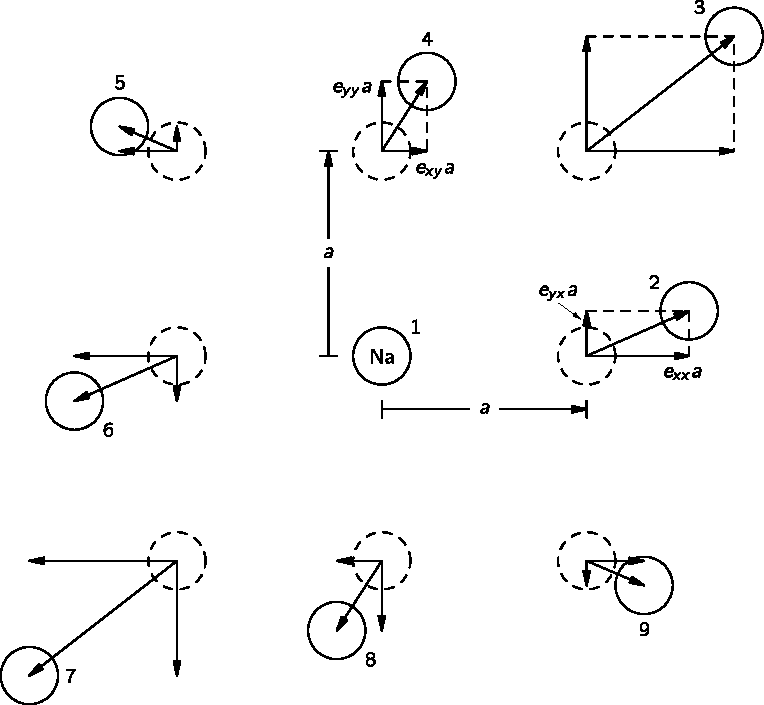
\includegraphics[width=0.7\linewidth]{fyz_fig0798.pdf}
      \caption{
               (\cite[s.~707]{Feynman02})}
      \label{fyz:fig0798}
    \end{figure}

    \todo[inline]{Kapitola fey2ch39 je nedodělaná, obsahuje pouze obrázky}
%} %tikzset
%---------------------------------------------------------------------------------------------------